\begin{section}{Resultados}

	Para analizar las diferencias y/o similitudes en la aplicación práctica de los tres algoritmos implementados se generaron gráficos que pasan a detallarse a continuación. 
		
	El primero de ellos consiste en gráficar el error relativo en función de la cantidad de iteraciones para cada uno de los algoritmos. Se utilizó precisión fija de 51 bits, con truncamiento. En el eje $y$ del siguiente gráfico se utilizó escala logarítmica (Figura \ref{fig:errorRelativo_elemSerie}).

		\begin{figure}[H]
			\centering
			\includegraphics[scale=0.5]{graficos/comparacion_42it.eps}
			\caption{Gráfico del error relativo en función de la cantidad de elementos en la serie}
			\label{fig:errorRelativo_elemSerie}
		\end{figure}

	/graficos/comparacion_42it.eps PEGAR EL FUCKING GRAFICO!!!!!!

	El error relativo del algoritmo de Gregory disminuye de forma logarítmica. Los dos algoritmos restantes, poseen pendiente negativa siendo la diferencia entre ellas, a priori, baja.

	El siguiente gráfico SOIDAJFOIDSAJFOISADJOIFJSODIJ

	Nota: No se utilizaron polinomios interpoladores para aproximar por la curva o recta que pase por todos los puntos correspondiente a una misma fuente de datos, estas conclusiones fueron sacadas utilizando experimentación empírica, suponiendo que el comportamiento cuando los valores del eje $x$ tienden a infinito se corresponden a los de los valores graficados.

\end{section}
